\subsubsection{Implementation of the wishbone interface (Jacob)} 
\paragraph{Requirements to fulfil}
FR.3.b.i
\paragraph{Theory}\mbox{}
\subparagraph{Pin Budget}
There is of cause a limited amount of GPIO pins available at the FPGA board, so a detailed pin budget will be made, to clarify how many pins are needed and which function each pin will have. This is essential to design the modules inside the FPGA, or at least to make them work prober without much confusion.


\begin{figure}[H]
\centering
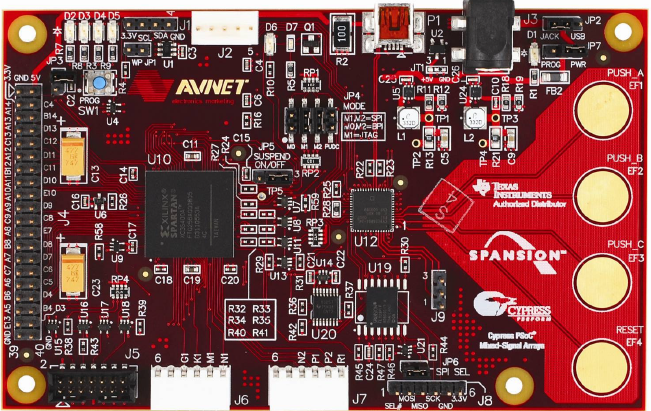
\includegraphics[width=\textwidth]{./Spartan3Aboard}
\caption{Spartan 3A board}
\label{fig:Spartan3Aboard}
\end{figure}




Figure \ref{fig:Spartan3Aboard} shows the layout of the Spartan 3A board. The pin connectors J4, J6 and J7 will be used. For the CPU interface, only J4 will be used. 

%DATA
\begin{table}[H]
\begin{center}
\caption{Data Pins}
\begin{tabular}{|l|l||l|l||l|}
\hline FPGA & FPGA & LPC & LPC & FUNCTION \\ 
PIN \# & PIN & PIN\# & PIN & \\
 & NAME &  & NAME & \\
\hline J4 4 & C4 & J2 60 & BD0 & DATA\_PIN0 \\ 
\hline J4 5 & A14 & J2 58 & BD2 & DATA\_PIN2 \\ 
\hline J4 6 & B14 & J2 56 & BD4 & DATA\_PIN4 \\ 
\hline J4 7 & A13 & J2 54 & BD6 & DATA\_PIN6 \\ 
\hline J4 8 & D13 & J2 52 & BD8 & DATA\_PIN8 \\ 
\hline J4 9 & C13 & J2 50 & BD10 & DATA\_PIN10 \\ 
\hline J4 10 & C12 & J2 48 & BD12 & DATA\_PIN12 \\ 
\hline J4 11 & A12 & J2 46 & BD14 & DATA\_PIN14 \\ 
\hline J4 12 & D11 & J2 59 & BD1 & DATA\_PIN1 \\ 
\hline J4 13 & B12 & J2 57 & BD3 & DATA\_PIN3 \\ 
\hline J4 14 & C11 & J2 55 & BD5 & DATA\_PIN5 \\ 
\hline J4 15 & A11 & J2 53 & BD7 & DATA\_PIN7 \\ 
\hline J4 16 & D10 & J2 51 & BD9 & DATA\_PIN9 \\ 
\hline J4 17 & A10 & J2 49 & BD11 & DATA\_PIN11 \\ 
\hline J4 18 & E10 & J2 47 & BD13 & DATA\_PIN13 \\ 
\hline J4 19 & A9 & J2 45 & BD15 & DATA\_PIN15 \\ 
\hline 
\end{tabular} 
\label{table:datatab} %\ref{table:datatab}
\end{center}
\end{table}

Table \ref{table:datatab} shows the data pins connections. Referring to  FR 3.a.i \& FR 3.b.i, 16 pins are reserved for the data transfer. 


%ADRESS
\begin{table}[H]
\begin{center}
\caption{Adress Pins}
\begin{tabular}{|l|l||l|l||l|}
\hline FPGA & FPGA & LPC & LPC & FUNCTION \\ 
PIN \# & PIN & PIN\# & PIN & \\
 & NAME &  & NAME & \\
\hline J4 20 & D9 & J2 42 & BA0 & ADDR\_PIN0 \\ 
\hline J4 21 & C9 & J2 40 & BA2 & ADDR\_PIN2 \\ 
\hline J4 22 & C8 & J2 38 & BA4 & ADDR\_PIN4 \\ 
\hline J4 23 & A8 & J2 36 & BA6 & ADDR\_PIN6 \\ 
\hline J4 24 & E7 & J2 34 & BA8 & ADDR\_PIN8 \\ 
\hline J4 25 & B8 & J2 41 & BA1 & ADDR\_PIN1 \\ 
\hline J4 26 & D8 & J2 39 & BA3 & ADDR\_PIN3 \\ 
\hline J4 27 & A7 & J2 37 & BA5 & ADDR\_PIN5 \\ 
\hline J4 28 & D7 & J2 35 & BA7 & ADDR\_PIN7 \\ 
\hline J4 29 & C7 & J2 33 & BA9 & ADDR\_PIN9 \\ 
\hline 
\end{tabular} 
\label{table:addrtab} %\ref{table:addrtab}
\end{center}
\end{table}

Table \ref{table:addrtab} shows the address pins used. 10 pins are reserved for address. 


\begin{table}[H]
\begin{center}
\caption{Motor Control Pins}
%MOTOR CONTROL
\begin{tabular}{|l|l||l|}
\hline FPGA & FPGA &  FUNCTION \\ 
PIN \# & PIN & \\
 & NAME & \\
\hline J4 31 & A6 & M\_CTRL4 \\ 
\hline J4 32 & C5 & M\_CTRL3 \\ 
\hline J4 33 & B6 & M\_CTRL2 \\ 
\hline J4 34 & D4 & M\_CTRL1 \\ 
\hline 
\end{tabular} 
\label{table:mctrltab} %\ref{table:mctrltab}
\end{center}
\end{table}

Table \ref{table:mctrltab} shows the four pins reserved for motor control. 4 output signals to two H-bridges, to control the motors position. One pin for each direction the solar panel has to move; up, down, left right. 


\begin{table}[H]
\begin{center}
\caption{LPC/FPGA Control Pins}
%LPC/FPGA CONTROL
\begin{tabular}{|l|l||l|l||l|}
\hline FPGA & FPGA & LPC & LPC & FUNCTION \\ 
PIN \# & PIN & PIN\# & PIN & \\
 & NAME &  & NAME & \\
\hline J4 35 & A5 & J1 45 & 2.14 & Chip Select \\ 
\hline J4 36 & B4 & J1 6 & Reset\_out & Reset \\ 
\hline J4 37 & E13 & J1 35 & BWE & Write Enable \\ 
\hline J4 38 & D3 & J1 36 & BOE & Output Enable \\ 
\hline 
\end{tabular} 
\label{table:lpctab} %\ref{table:lpctab}
\end{center}
\end{table}

Table \ref{table:lpctab} shows the chip select, which has to be high for the FPGA to react on commands from the LPC, Reset for a synchronous reset of both boards. When reset is pressed on the LPC board, Reset\_out will be set low, which the FPGA will react on. Also if the power is lost, the pin will go low, and secure a reset/idle state, until the power is turned on again. Also the Write and Read enable are described, for the LPC to control whether the FPGA has to send or receive data from the LPC. 


\begin{table}[H]
\begin{center}
\caption{LPC Control Pins}
%LPC/FPGA CONTROL
\begin{tabular}{|l||l|l||l|}
\hline  Connection 	& LPC 	& LPC 	& FUNCTION \\ 
 	 				& PIN\# & PIN 	& \\
 	 				&  		& NAME 	& \\
\hline  Chip Select	& J2 43 & DBUS\_EN & Data Bus Enable \\
\hline  Ground		& J2 44 & ABUF\_EN & Address Buffer Enable \\
\hline 
\end{tabular} 
\label{table:bustab} %\ref{table:bustab}
\end{center}
\end{table}

Table \ref{table:bustab} shows that DBUS\_EN is connected to Chip Select. This is enabled when chip select is enabled. This data bus is controlled by the WE and OE signals, and can act both as input and output. This should not be left low, else it will collide with the boards internal data bus, therefore it is connected to Chip Select, and is only low when chip select is enabled. DBUS\_EN is active low. \\
ABUF\_EN is grounded, to pull it low constantly. This will enable the two buffers for address. Also the control signals are enabled, and act as output. [LPC2478\_OEM\_Board\_Users\_Guide\_Rev\_H, page 10, chap 3.1.6] 


\begin{table}[H]
\begin{center}
\caption{Others}
%OTHERS
\begin{tabular}{|l|l||l|}
\hline FPGA & FPGA & FUNCTION \\ 
PIN \# & PIN & \\
 & NAME & \\
\hline J4 1 & GND & GND \\ 
\hline J4 2 & +5V & +5V SUPPLY \\ 
\hline J4 3 & +3.3V & +3.3 SUPPLY \\ 
\hline J4 30 & C6 & FREE \\ 
\hline J4 39 & GND & GND \\ 
\hline J4 40 & GND & GND \\ 
\hline 
\end{tabular} 
\label{table:otherstab} %Uset to refer to table: \ref{table:otherstab}
\end{center}
\end{table}
A lot of text, to describe the table of data!




\subparagraph{State Machine Diagram (Jacob)}
Before implementing the VHDL code, a state machine diagram is made to clarify which states the module has to go through. When this is in place, the code is very easy to implement.
\begin{figure}[H]
\centering
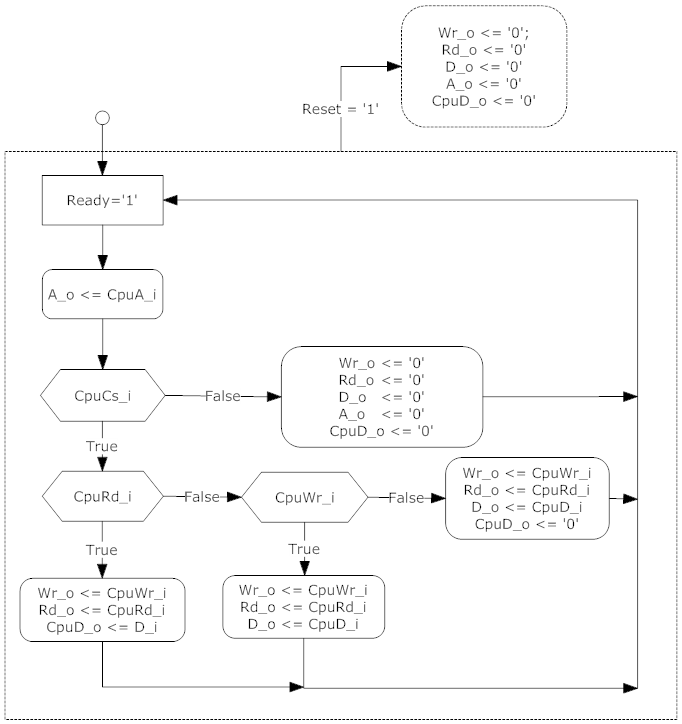
\includegraphics[width=10cm]{./State_Machine_Diagram_CpuInterface_v0_9}
\caption{State Machine Diagram - CpuInterface}
\label{fig:State_Machine_Diagram_CpuInterface_v0_9}
\end{figure}
Figure \ref{fig:State_Machine_Diagram_CpuInterface_v0_9} shows the State MAchine Diagram for the CpuInterface. The different states will be discussed in the "implementation" chapter below.

\paragraph{Implementation}\mbox{}\\
Important thing first. The module has to check if the reset pin is enabled. If this is the case, it has to reset the board, no matter what. This is why it is set asynchronious. No clock has to be on its rising or falling edge. The reset values is all 0, to be sure no data is stored, no adress is stored and no write/read commands are given to the Wishbone Master. 
\begin{verbatim}
-- Check if reset=high (Unsynchronized)

	-- Reset all values to '0'

	if(Rst='1') then

		Wr_o <= '0';

		Rd_o <= '0';

		D_o <= (others => '0');

		A_o <= (others => '0');

		CpuD_o <= (others => '0');
\end{verbatim}

If reset is not set, the module has to think syncronous. This is why we check the clock. Both the read and write state is inside the synchronous clock state, and also the chip select (CpuCs\_i) has to be high, in order for the module to respond on read/write commands. When chip select is set high, the adress is sent from the Cpu to the Wishbone Master. The adress can always be set, without any failures occur.\\
Then it is time to check if the "Read" is set. If it is, then the CPU wants to read data from the FPGA, thats why the data from the Wishbone master (D\_i) is sent to the output to the cpu (CpuD\_o).\\
Also the Read and Write input from the cpu is sent to the wishbone master. Then the cpu will have to avoid both being high at the same time. 
\begin{verbatim}
	elsif(Clk'event and Clk = '1') then --(All sync)	

	-- Check if active read (CPU read ffrom FPGA)

		if(CpuCs_i = '1') then

		A_o <= CpuA_i; -- Common for all

			if(CpuRd_i = '1') then

				Wr_o <= CpuWr_i; 	-- Enables/Disables master write

				Rd_o <= CpuRd_i; 	-- Enables/Disables master read

				CpuD_o <= D_i;		-- Data from master (D_i) to CPU (CpuD_o)
\end{verbatim}

If read is not high, the write pin has to be checked. If that is enabled, the CpuInterface will send the data recieved from the Cpu to the Wishbone master. Again both read and write is rooted directly to the Wishbone Master.
\begin{verbatim}
			-- Check if active write (CPU write to FPGA)

			elsif(CpuWr_i = '1') then

				Wr_o <= CpuWr_i;	

				Rd_o <= CpuRd_i;

				D_o <= CpuD_i;		-- Data from CPU (CpuD_i) to Master (D_o)

			else
\end{verbatim}


If either read nor write is high, the Cpuinterface will reset the Cpu data out to all "0". Also the read and write are directly rooted to the wishbone master, which also is "0". This will keep the system from making any action when not supposed to. 
\begin{verbatim}
			-- Reset values to 0

				Wr_o <= CpuWr_i;

				Rd_o <= CpuRd_i;

				D_o <= CpuD_i;

				CpuD_o <= (others => '0');

			end if;
\end{verbatim}

Last but not least, if chip select is not enabled, all values will be reset, as iff the reset button was pressed. This is to avoid any failures and unwanted actions in the system. 
\begin{verbatim}
		-- If Chip not selected (CpuCs_i = '0'), reset all values to '0'.

		else 

			Wr_o	<= '0';

			Rd_o 	<= '0';

			D_o	<= (others => '0');

			A_o	<= (others => '0');

			CpuD_o <= (others => '0');

		end if;

	end if;
	end process Cpuinter;
\end{verbatim}

\paragraph{verification of requirements}\mbox{}\\


\subsubsection{Module Design (Jacob)} 
\paragraph{Requirements to fulfil}\mbox{}\\
NR.4.b\\
\paragraph{Theory}\mbox{}\\
The module design shall help us clarify which blocks shall be implemented where. All the hardware, the Spartan 3A board, the LPC2478 and other modules, shall be drawn an connected. This clarifies what the different hardware contains and how they interface with each other. The module design is shown in Figure \ref{fig:module_design_v0_9}

\begin{landscape}
\begin{figure}[h!]
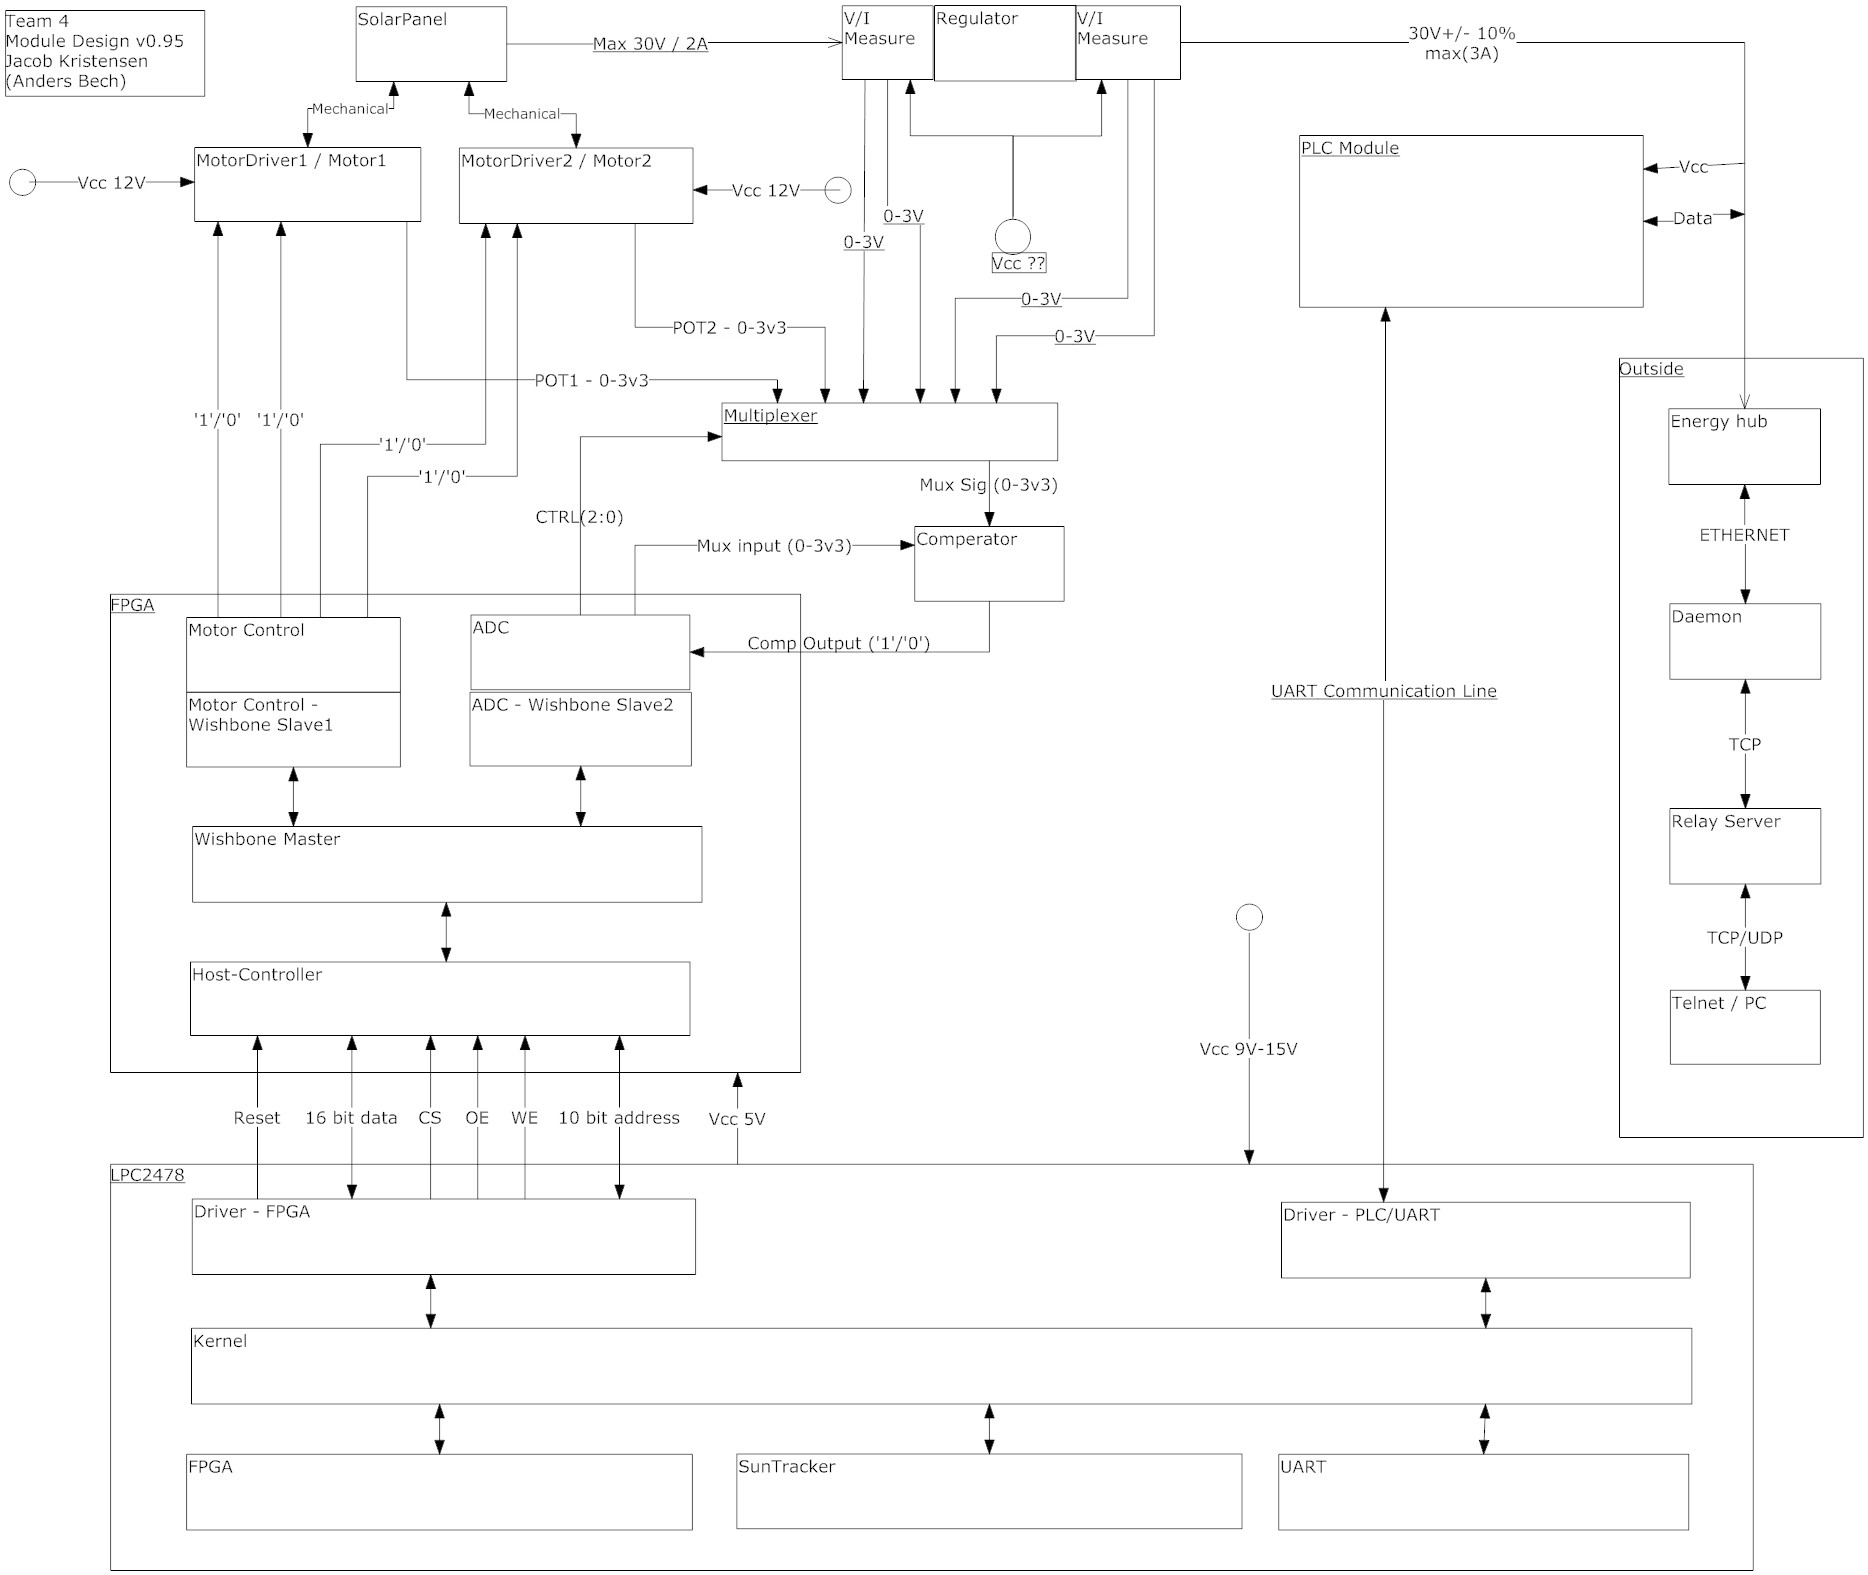
\includegraphics[width=20CM]{./module_design_v0_9_5}
\caption{Module Design of "system-to-be"}
\label{fig:module_design_v0_9}
\end{figure}
\end{landscape}

The \textbf{solar panel} is physically connected to the two motors, which will turn the panel towards the sun. \textbf{The two motors} are each supplied by 12 V DC (Source unknown). Four signals are received from the \textbf{FPGA}, that controls which way the motors have to turn. Those signals are sent to two H-bridges, which will invert the voltage, and make the motors turn in different directions. The four signals are controlled by a \textbf{PWM} block in the FPGA, to make speed control of the motors possible. \\
The potentiometers of the motors will return a value to the \textbf{ADC} implemented in the FPGA, which then can compare their position, to the position of the sun, received from the LPC2478. The ADC input limit, on the FPGA board is 3v3\footnote{FPGA datasheet page 3.}\\
The ADC and the PWM are implemented in a wishbone structure, which makes it possible to use it at different platforms, if the wishbone interfaces are obeyed. The two wishbone slaved (PWM, ADC), are interfaced to the LPC2478 through a wishbone master, controlling the communication, and then through a host-controller, onto the FPGA-driver implemented on the LPC2478 board. \\
The SPARTAN 3A board and the LPC2478 developers kit is a requirement to this project, given by the teachers. The \textbf{FPGA} board is software coded hardware, which means it makes most sense to replace some actual hardware by this development board, or maybe make a module more efficient, by replacing some of the software by this "hardware" board. In this case it is replaced by both. The suntracker was meant as pure software, but now a formula, calculating the position of the sun, is implemented as software, and the position of the sun is sent to the FPGA; which compares it to the position of the motors, received by the potentiometers, and then repositioning the motors, according to the sun. \\
The \textbf{LPC2478} board is where the software is placed, and are an essential part of the system. This is used for communication, logging and other things, which will be described later. The board is controlled by a small embedded Linux system. Three drivers are implemented, and they are controlled by the kernel, on behalf of three user applications. This board is supplied with a voltage between 9-15V DC\footnote{LPC2478 print}. \\
The first interface was the interface for communication with the FPGA, shortly described above. This is a 16 bit communication line, which is also a requirement for the system. Further there is a chip select, read and write line and finally a supply line, supplying the FPGA with power from the LPC2478 board\footnote{LPC2475 user manual, chap. 5 - External Memory Controller}. The FPGA user application will handle the information that is to be sent and received. \\
The power generated from the solar panel, will be sent through a \textbf{regulator}, which is pure hardware, where the power will be converted from approx 30V, into 30V+/-10\%. This output is a common requirement, to make the system function with the other systems. \\
Two galvanic isolated \textbf{sensors} are applied to the input and the output of the regulator, to keep track of how much energy is produced and how efficient the regulator is. Those sensors sends a PWM signal (0-3v)\footnote{LPC2478 user manual, chap 28.2} down to the ADC, in the sensor driver, in the LPC2478 board. The user application to the sensor driver will then pack the data and send them to the energy hub, which updates the web-page. \\
The last user application/driver at the LPC board is the \textbf{PLC driver}, which makes the communication to the energy hub possible. This communication is established through UART, which sends and receives messages between the system and the energy-hub. A\textbf{ PLC module} is implemented too, which is supplied by the powerline and speaks through it too. 

\paragraph{verification of requirements}\mbox{}\\
